\documentclass[a4paper,12pt]{article}
\usepackage[utf8]{inputenc}
\usepackage[french]{babel}
\usepackage[T1]{fontenc}
\usepackage{graphicx}
\usepackage{hyperref}
\usepackage{float}
\usepackage{glossaries}
\usepackage{csquotes}

\usepackage[
backend=biber,
style=numeric,
sorting=ynt
]{biblatex}

\addbibresource{parties/biblio.bib}

\makeglossaries

\graphicspath{ {./image/} }

\usepackage{lmodern,tikz,lipsum}
\usepackage[a4paper,
            bindingoffset=0.2in,
            left=1in,
            right=1in,
            top=1in,
            bottom=1in,
            footskip=.25in]{geometry}

\newcommand\framethispage[1][2cm]{%
    \tikz[overlay,remember picture,line width=2pt]
    \draw([xshift=(#1),yshift=(-#1)]current page.north west)rectangle
         ([xshift=(-#1),yshift=(#1)]current page.south east);%
}

\usepackage{wrapfig}
\usepackage{threeparttable} 


\usepackage{lipsum}
    
\begin{document}

\newcommand\interline{0.3cm}
\thispagestyle{empty}
%\fbox{
%\begin{minipage}{\textwidth}
\begin{titlepage}
\framethispage[1.9cm]% le cadre est à 2 cm des bords de la feuille
\begin{center}

\vspace{1cm}
\begin{minipage}[b]{3.5cm}

\includegraphics[width=2cm]{LOGO_RVB_grand-UM.jpg}
\end{minipage}\begin{minipage}[b]{3.5cm}


\includegraphics[width=2cm]{lirmm.fr.png}
\end{minipage}\begin{minipage}[b]{3.5cm}


\includegraphics[width=2cm]{logo.png}
\end{minipage}\begin{minipage}[b]{3cm}


\includegraphics[width=2cm]{LOGO_DTP_INFORMATIQUE.jpg}
\end{minipage}
\vspace{1cm}

\Large{Université de Montpellier\\
\vspace{\interline}

Faculté des Sciences} \\
\vspace{2cm}

{\huge MASTER 2 INFORMATIQUE \\
\vspace{\interline}

Parcours IMAGINE \\}
\vspace{2cm}
{\huge \textbf{Automatisation du prétraitement de photos de mandrills}}\\
\vspace{2cm}
Effectué au LIRMM et au CNRS \\
\vspace{\interline}
du 31 janvier au 29 juillet 2022 \\
\vspace{\interline}
par Maxime BOUCHER\\
\vspace{2cm}
Tuteurs en entreprise: William Puech et Julien Renoult \\
\vspace{\interline}
Tuteur à l'université: Madalina Croitoru 
\end{center}
\end{titlepage}


\newglossaryentry{tensorflow}
{
    name=tensorflow,
    description={Tensorflow est une librairie Python de Google, écrite en C++, qui permet d'écrire des réseaux de neurones avec une API assez haut niveau}
}

\newglossaryentry{ReLU}
{
    name=ReLU,
    description={La fonction d'activation ReLU est une fonction composée, linéaire sur $[0, \infty]$ et nulle sur $[-\infty, 0]$. Elle est donc non linéaire et permet aux réseaux de neurones d'être plus précis}
}

\newglossaryentry{kanban}
{
    name=kanban,
    description={Un kanban est un tableau où figurent multiples colonnes à étiquettes. Le développeur saisit une tâche, par exemple, dans la colonne TODO et la place dans DOING. Les autres développeurs voient alors que cette dernière est déjà en cours d'accomplissement. Enfin, une fois la tâche finie, le développeur la place dans une colonne DONE. On peut étendre ce système de méthode AGILE avec un système de peer-reviewing, où une fois une tâche accomplie, elle doit être vérifiée par un pair avant d'être réellement acceptée}
}

\newglossaryentry{matrice de confusion}
{
    name=matrice de confusion,
    description={Une matrice de confusion permet d'étudier les prédictions d'un modèle. L'accuracy, seule, n'est pas assez utile pour juger un modèle de classification. Car un modèle peut, dans un contexte d'imbalance des classes, toujours prédire la même chose et avoir une excellente accuracy. La matrice de confusion affiche quant à elle l'efficacité du modèle par classe, et donc permet de savoir si le modèle est aussi efficace sur chacune d'entre elles ou non}
}

\newglossaryentry{transfer learning}
{
    name=transfer learning,
    description={Le transfer learning est une méthode en machine learning pour réutiliser le travail déjà effectué. En effet, un réseau de neurones apprend à déceler des features : par exemple, la forme des yeux. Une fois entrainé, on va sauvegarder ces poids et potentiellement le distribuer sur Internet pour que d'autres puissent extraire ces features en réutilisant les poids sauvegardés. Ensuite, on peut spécialiser le réseau de neurones pour l'adapter à un problème qui serait similaire}
}

\newglossaryentry{classification}
{
    name=Classification,
    description={Une classification est une résolution d'un problème en machine learning où l'on veut prédire si une donnée en entrée appartient à une classe ou une autre. C'est une sorte de régression avec une sortie discrète plutôt que continue. C'est notamment utilisée pour le tagging dans la photographie (cet animal est-il un chat ou un chien?)}
}

\newglossaryentry{docker}
{
    name=docker,
    description={Docker est un logiciel qui permet de lancer un processus isolé et restreint. Ainsi, on peut utiliser Docker pour lancer des logiciels avec leurs propres versions de librairies. Par ailleurs, Docker utilise généralement Linux en OS host, donc c'est adapté à une utilisation, que ce soit en développement, production, petits ou gros systèmes..}
}

\newglossaryentry{accuracy}
{
    name=accuracy,
    description={L'accuracy est une mesure qui décrit le taux de de prédictions correctes.
    \begin{equation}
        accuracy = \frac{nombre de prédictions correctes}{nombres d'échantillons}
    \end{equation}}
}

\newglossaryentry{XMP}
{
    name=XMP,
    description={Les métadonnées XMP sont des métadonnées liés intrinsèquement à Adobe Lightroom. Elle permet de rajouter des tags dans le champs Keywords, que l'on utilisera pour stocker tous les différents labels qui seront utilises pour nos modèles de machine learning}
}

\newglossaryentry{oversampling}
{
    name=oversampling,
    description={L'oversampling est une méthode qui implique la génération d'images pour égaliser le nombre d'échantillons entre différentes classes, dans le cadre d'une classification (ou même d'un régression en théorie même s'il n'y a pas de classes). Diverses méthodes existent, et j'en ai créée une qui semble être bien adapté à notre problème en particulier, qui est décrite dans les réalisations}
}

\newglossaryentry{courbe ROC}
{
    name=courbe ROC,
    description={La courbe ROC permet d'étudier ici le taux de vrais positifs en fonction du taux de faux positifs, pour chaque classe}
}

\newglossaryentry{SQLite}
{
    name=SQLite,
    description={Une base de données SQLite est une base de données relationnel sans serveur (basé sur un fichier seul à la manière d'un CSV par exemple). C'est assez facile à partager ou gérer dans un laboratoire non spécialisé en informatique, tout en ayant un avantage certain en performances et robustesse comparé à une solution comme des fichiers CSV}
}

\newglossaryentry{CSV}
{
    name=CSV,
    description={Un fichier comma separated values (CSV) est un tableau dont chaque colonne est séparer par une virgule, et chaque ligne par un retour à la ligne}
}

\newglossaryentry{dataset}
{
    name=dataset,
    description={Un dataset est un ensemble de données. Dans notre cas, un dataset est un ensemble d'images (de mandrills) et de leurs labels associés (FaceQual pour n'en citer qu'un). En machine learning, on doit avoir les valeurs X, ici les images, et les valeurs Y, ici leur label, pour ensuite que le modèle fasse une régression de la fonction et puisse ensuite, à partir d'une nouvelle image X et de son entraînement, prédire leur label Y}
}

\newpage

\newpage

\renewcommand{\contentsname}{Table des matières}

\tableofcontents

\newpage


\newpage

\section{Remerciements}
Je tiens à remercier Monsieur Julien Renoult, chargé de recherche au CNRS, qui a co-encadré mon stage, et m'a énormément guidé dans mes actions et m'a fait confiance tout au long de cette période.
\newline

Je remercie également M. William Puech, professeur des universités et chercheur au LIRMM, qui, en tant que co-encadrant du stage, a porté un regard critique et bienveillant sur mes travaux. Je n'oublie pas ses nombreux conseils.\newline

Je remercie particulièrement Mme Claudia Ximena Restrepo-Ortiz, ingénieure en bioinformatique, ma tutrice opérationnelle sur le projet, qui a dirigé mes expérimentations de manière optimale, et m'a aidé dans ma façon de présenter les résultats des expérimentations.\newline

Je remercie également Mme Sonia Mai Tieo, experte en Intelligence Artificielle au CNRS, pour ses nombreux conseils, et son aide dans l'appréhension de la discipline.\newline

J'adresse également mes remerciements à ma tutrice côté Université, Mme Madalina Croitoru, avec qui je faisais des points réguliers, qui m'ont permis d'aborder ce stage en toute confiance.\newline

Et enfin, je remercie mon référent pédagogique, M. Pierre Pompidor, pour son aide efficace dans les démarches de recherche de stage et son suivi. 
\newline

\newpage
\section{Introduction}
Il s'agit d'un stage dans le domaine de l'intelligence artificielle, co-encadré par deux laboratoires, le LIRMM et le CEFE, grâce à une bourse de Master interdisciplinaire du projet MUSE. \newline

Le projet MUSE « Montpellier Université d’Excellence » vise à faire émerger à Montpellier une université thématique de recherche intensive, internationalement reconnue pour son impact dans les domaines liés à l’agriculture, l’environnement et la santé.\newline

Le stage dure du 31 février au 29 juillet 2022, il se déroule au sein du projet "Mandrillus".\newline

Le projet Mandrillus, né en 2012 et dirigé par Mme Marie Charpentier (CNRS), se déroule principalement dans la réserve de Lékédi au Gabon, et a pour objectifs:
\begin{itemize}
    \item d'obtenir des informations sur la vie et l'écologie des Mandrills
    \item d'aider à la protection des Mandrills
    \item de soutenir les populations locales\newline
\end{itemize}


Depuis 2012, l’équipe a rassemblé plus de 30,000 portraits de mandrills issus d'une population de prêt de 300 individus. L'équipe sur le terrain produit aujourd'hui prêt de 2,000 nouvelles images par mois.\newline

L'objectif de ce stage est de concevoir des algorithmes qui permettront, au final, d'automatiser la reconnaissance des individus et l'annotation des nouvelles images. Pour cela, il faut d'abord concevoir les traitements intermédiaires qui permettront d'atteindre l'objectif final:  
\begin{itemize}
    \item évaluation de la qualité des photos, si le mandrill présent sur cette dernière est de face ou de profil, en vue d'un tri pour des usages a posteriori.
    \item évaluation de l'âge des mandrills à partir de leur photographie.
    \item éventuellement, mise au propre / uniformisation du code pour une meilleur maintenance
\end{itemize}
\newpage
\section{Présentation de l'entreprise} 

\subsection{Le CNRS - CEFE}

Le centre d'écologie fonctionnelle et évolutive (CEFE) est un centre de recherche du CNRS dédié à l'écologie. Pour citer leur résumé sur leur site web \cite{cefe}: 
Le projet du CEFE vise à comprendre la dynamique, le fonctionnement et l’évolution du vivant, de «la bactérie à l’éléphant », et « du génome à la planète ». Il s’appuie sur trois ambitions : [1] comprendre le monde vivant pour anticiper ce que sera demain, [2] conduire à des innovations et répondre aux attentes de la société ; [3] pratiquer une science « rassembleuse » et diverse dans ses approches disciplinaires. Les questions de recherche sont posées dans un contexte marqué par la prégnance des changements planétaires, le développement de nouvelles technologies de manipulation du vivant, et l’exigence croissante de la société pour la recherche.\newline
(...)\newline
Le CEFE est organisé en quatre départements scientifiques entourés de plates-formes techniques communes. 

\begin{itemize}
    \item Ecologie Evolutive et Comportementale
    \item Dynamique et Conservation de la Biodiversité
    \item Ecologie Fonctionnelle
    \item Interactions, Ecologie et Sociétés \\
\end{itemize}

Au sein du CEFE, l'aile E3CO (Ecologie Evolutive Empirique, Communication \& Coopération) est quant à elle consacrée à l'étude de l'écologie évolutive et comportementale, dédié aux êtres vivants.
L'équipe dirigée par Julien Renoult travaille, entre autres, sur le projet Mandrillus, auquel j'ai participé.

\subsection{Le LIRMM}

Le laboratoire d'informatique, de robotique et microélectronique de Montpellier qui est une collaboration entre le CNRS et l'université de Montpellier.
J'ai été plus précisément affecté à l'équipe ICAR, qui travaille sur la compression d'images, la sécurité et la 3D principalement.\newline

L’équipe ICAR (Image \& Interaction) regroupe des chercheurs des deux départements Robotique et Informatique autour de la thématique « image » et plus généralement des données visuelles. Elle est composée actuellement de neufs permanents, universitaires et CNRS mais compte aussi dans ses collaborateurs réguliers, plusieurs médecins hospitalo-universitaires du CHU utilisant l’imagerie médicale, des chercheurs en télédétection du laboratoire TETIS ou en modélisation pour l’agronomie du CIRAD.\newline

L’équipe ICAR développe des thèmes de recherche associant l’interaction et le traitement des données visuelles telles que les images 2D, 3D, multi-spectrales (nD), les vidéos ou les séquences d’images nD+t et les objets 3D que ce soit sous forme de maillages 3D ou de modélisations paramétriques.\newline

L’équipe est structurée suivant 4 axes de recherche : 
\begin{itemize}
    \item Analyse \& traitement
    \item Sécurité Multimédia
    \item Modélisation \& Visualisation
    \item Intelligence Artificielle pour les données visuelles
\end{itemize}


\section{Présentation de la mission (facultatif, nécessaire si la présentation du sujet dans l'introduction ne suffit pas) }


\section{Environnement technique} 
Je travaille sur un ordinateur fourni par le CNRS, avec, lorsque je suis au lirmm, une connexion à distance par Remote Desktop Protocol (RDP). J'utilise également mon ordinateur fixe sur lequel je me connecte en SSH. \\

À mon arrivé, le contrôle de versions n'existait pas. On a donc mis en place un projet Github versionné par Git, le standard pour le contrôle de versions décentralisés. \\

Pour le deep learning, Tensorflow (créé par Google) 2.X sera utilisé. C'est une des librairies majeurs en machine learning, avec PyTorch (créé par Facebook) pour concurrent. \\

Le choix d'ajouter Docker dans une partie du travail permet de s'affranchir en partie du problème de l'environnement technique, c'est-à-dire que l'environnement de l'utilisateur est différent de celui de développement et de production (dans notre cas, la production ne représente pas réellement quelque chose de séparé du développement mais on peut facilement imaginer qu'on veuille utiliser un ordinateur plus puissant, voire un supercalculateur, pour entrainer le réseau de neurones. Dans ce cas là, Docker permettrait que le code fonctionne sans problèmes).

\section{Veille technologique ou appropriation scientifique (facultatif)} 
Durant la période entre les derniers partiels et le début du stage, j'ai travaillé les différents tutoriels Tensorflow, et j'ai commencé à effleurer la théorie concernant le machine learning (descente de gradient...)\newline

Puis, pendant le stage, j'ai étudié des méthodes pour résoudre des problématiques spécifiques, comme le bruit de labellisation, ou encore l'ordonnancement des classes, en répertoriant des méthodes et en  mettant en pratique quelques unes. \newline

J'ai réalisé un état de l'art de la prédiction de l'âge à partir d'images de face (d'humains).

\section{Travaux effectués} 

\subsection{Classification des images par qualité, face profils}
L'objectif fixé à la première visio conférence a été déterminé : faire de la classification sur la qualité des photographies des mandrills.\\

J'ai donc commencé par faire du transfer learning avec MobileNet V2, un CNN existant de Google adapté aux mobiles (c'est-à-dire, très rapide et plutôt performant) pour essayer d'adapter un modèle avec les poids ImageNet pour la classification de la qualité des photographies. Notre dataset ressemble aux images ci-dessous, avec FaceQual0-3 en label de qualité, 3 étant la meilleure qualité.

\begin{center}
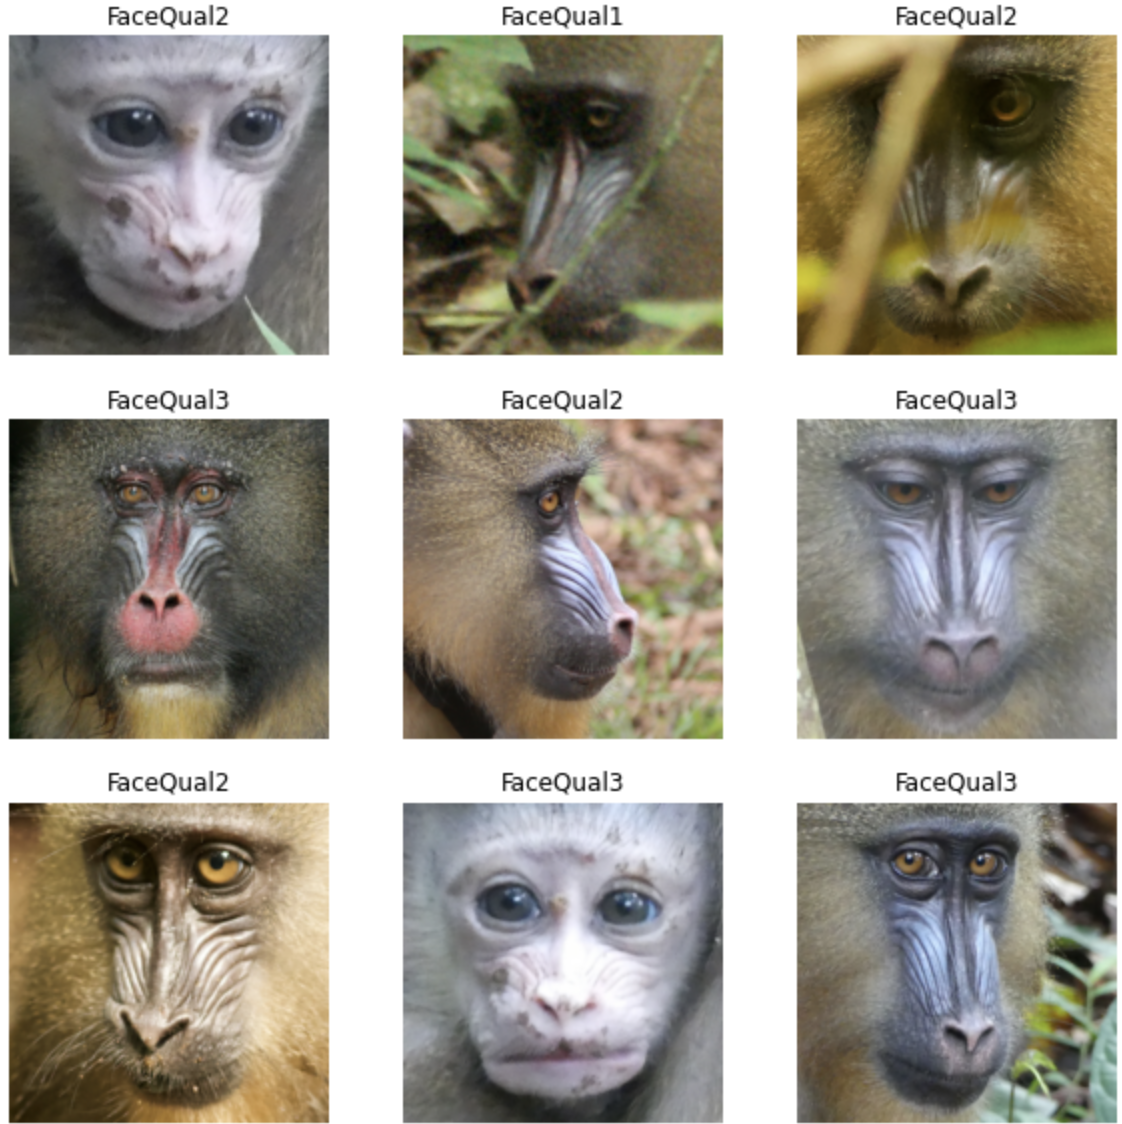
\includegraphics[width=200pt]{imgs/qualité/cr1/dataset.png}
\end{center}

Les premiers résultats semblent bons à première vue : 85\% d'accuracy sur une classification simple.

\begin{center}
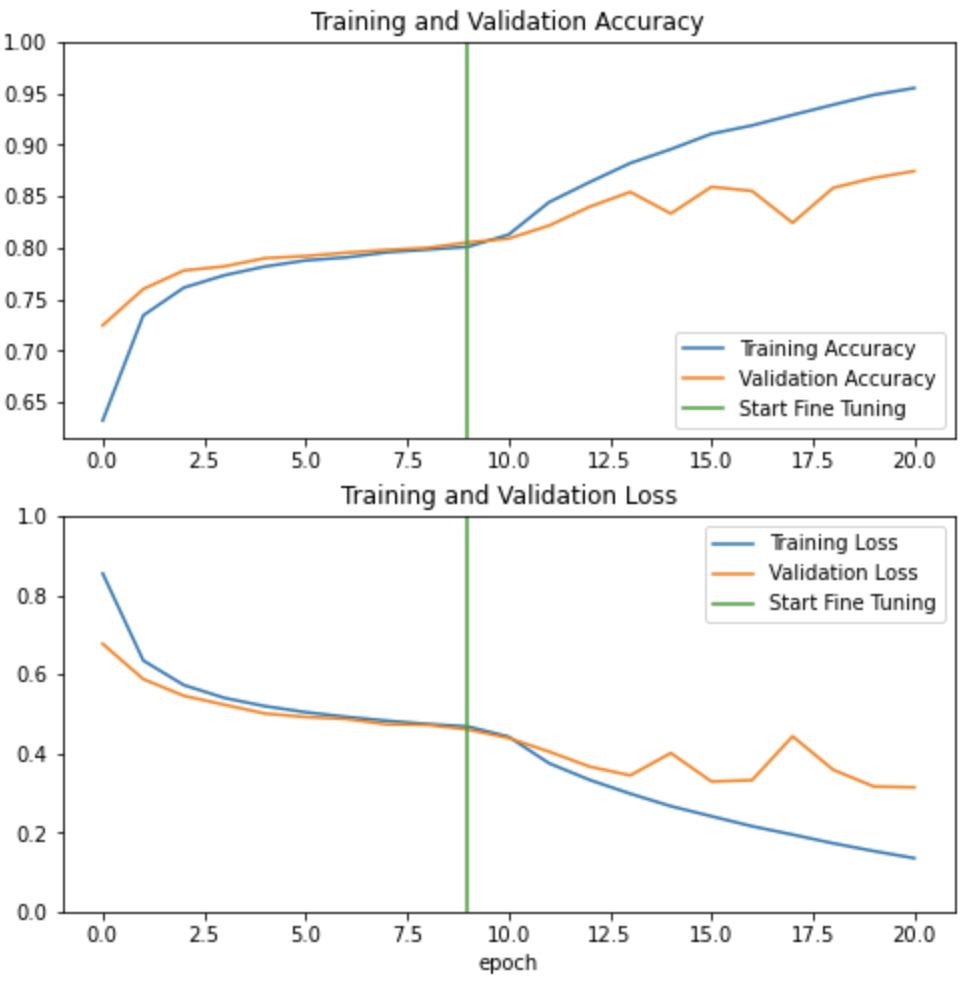
\includegraphics[width=200pt]{imgs/qualité/cr1/resultat1.png}
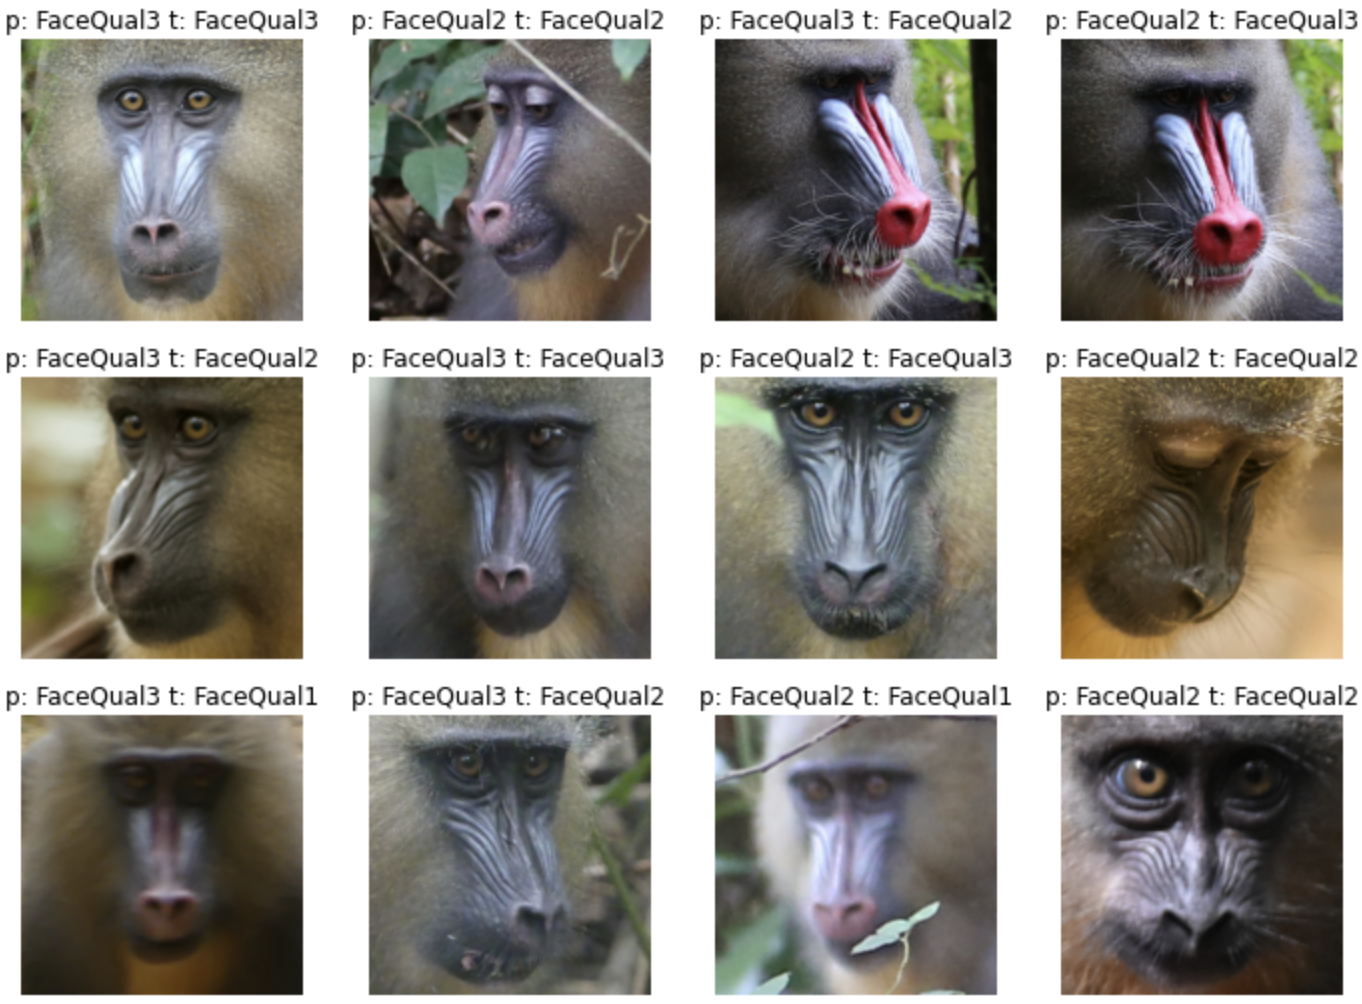
\includegraphics[width=200pt]{imgs/qualité/cr1/prediction1.png}
\end{center}

Mais les résultats sont trompeurs, en effet, le jeu de données est très déséquilibré, avec 10000 images de qualité FaceQual2 et 6000 de qualité FaceQual3 contre 250 et 1000 de qualité FaceQual0 et FaceQual1. Le modèle pourrait donc prédire tout le temps FaceQual2 et avoir 57\% d'accuracy par défaut.\\

Il faut donc gérer ce déséquilibre, et deux approches nous paraissent intéressantes :\\
\begin{itemize}
    \item dégrader des images de bonne qualité (downscale puis upscale et léger floutage) pour génerer des photos de mauvaises qualité (une mauvaise photo souvent a un manque de détails et/ou est flou).
    \item pondérer les classes de jeu de données pendant l'entrainement (accorder plus d'importance donc là où on aurait moins d'échantillons).
\end{itemize}

Voici un exemple de ce que pourrait être une dégradation d'images par rapport aux premières images :

\begin{center}
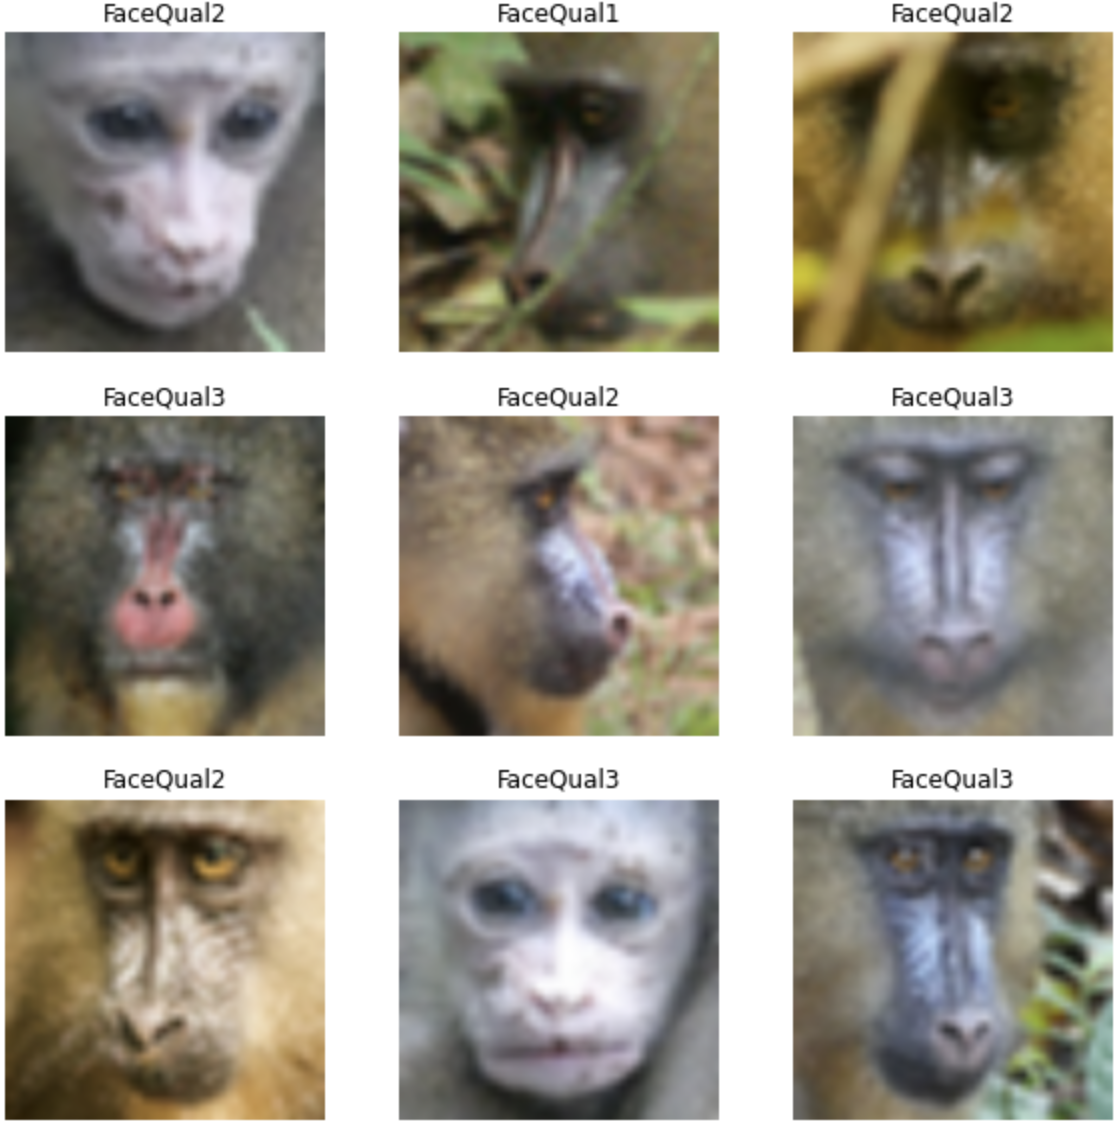
\includegraphics[width=200pt]{imgs/qualité/cr1/augmentation1.png}
\end{center}

Évidemment on peut faire varier le niveau de floutage et de dégradation de détails. On pourrait également imaginer appliquer un fort taux de compression JPEG ou augmenter le bruit artificiellement pour obtenir des images de basse qualité réalistes (tout cela étant des facteurs de basse qualité).\\

Ensuite, j'ai travaillé sur la matrice de confusion et le graphe ROC et commencer à comparer de manière plus complète les modèles.\\

Nous démarrons avec un transfer learning par VGG16/ImageNet suivi de deux couches complètements connectés, par enfin une couche softmax (probabilités).

Nous obtenons sur 10 epochs un rappel à 0.8 pour les 2 classes les plus représentés (FaceQual2/3) et 0.65 pour les autres (FaceQual0/1). Cela veut donc dire qu'une proportion correcte initiale d'échantillons est correctement classé.

\begin{center}
    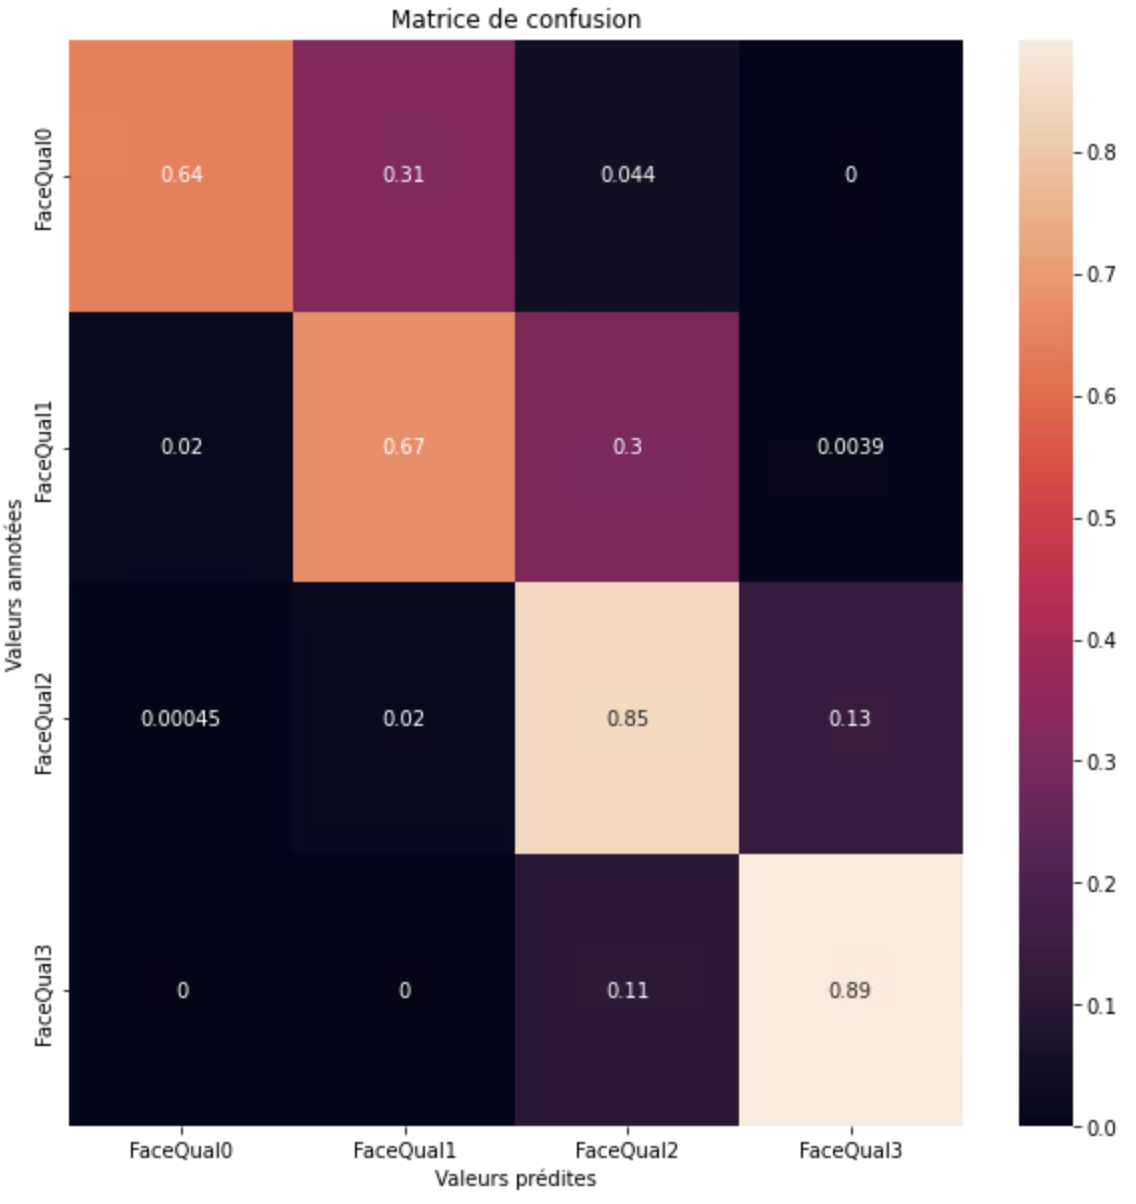
\includegraphics[width=170pt]{imgs/qualité/cr2/vgg16_000_confusion.png}
    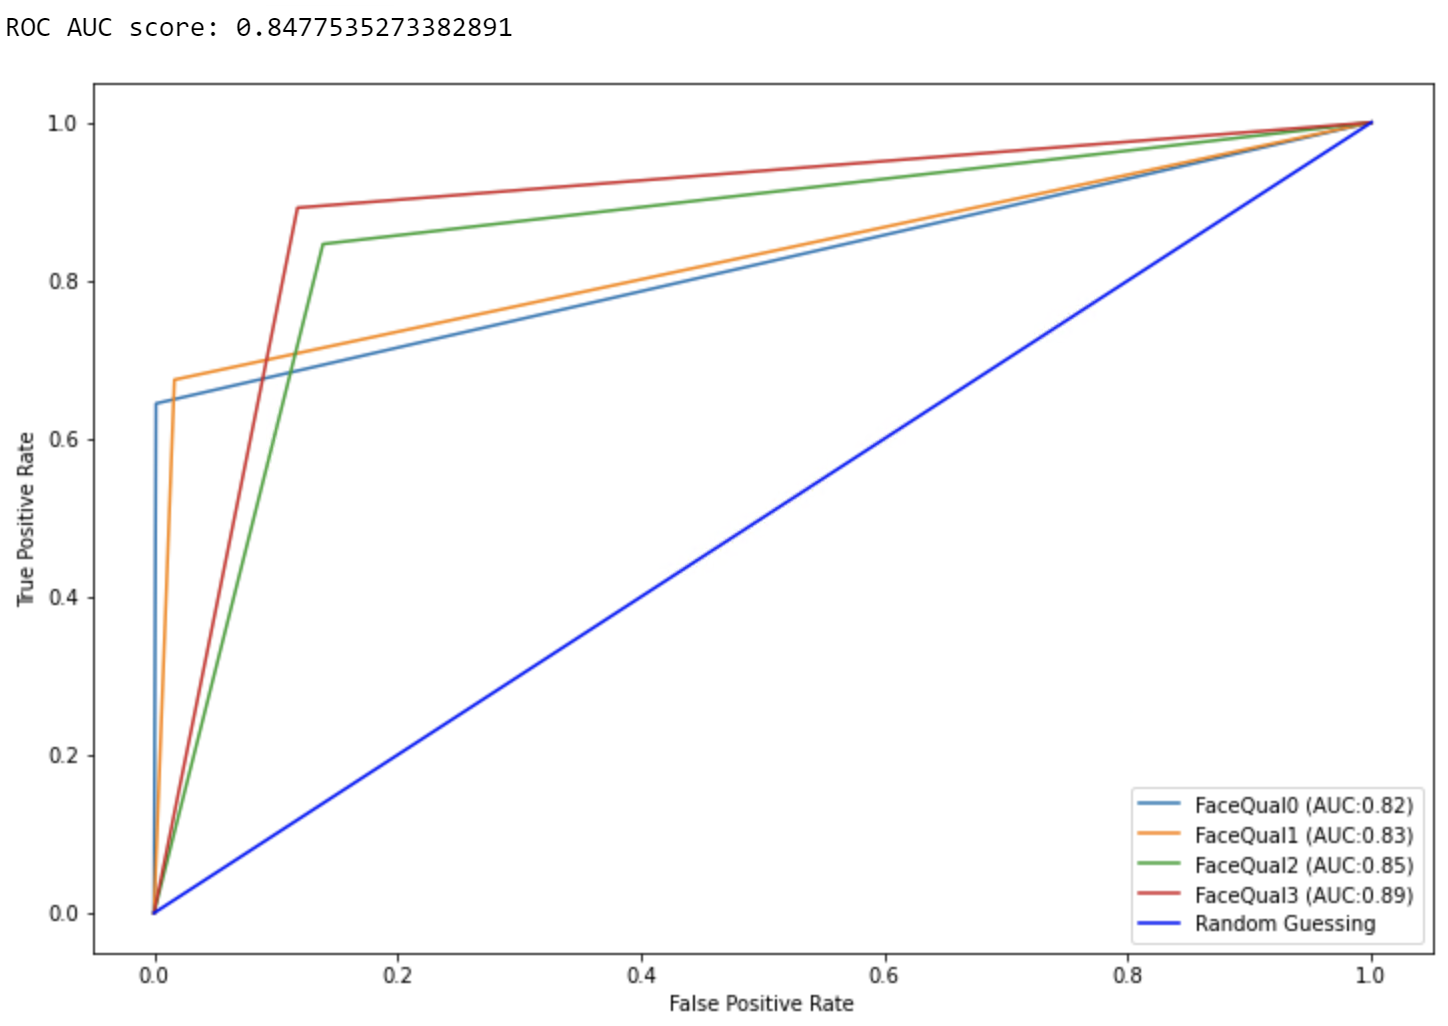
\includegraphics[width=170pt]{imgs/qualité/cr2/vgg16_000_roc.png}
\end{center}

Pour améliorer la situation, problématique sûrement à cause du déséquilibre des données, nous pouvons essayer d'abord la pondération des classes. Cela permet en effet d'améliorer largement le résultat de la classe la plus sous représentée (FaceQual0), avec un poids d'importance de 17. Seulement, une partie de l'apprentissage est troublée, d'une part car la classe FaceQual1 est partiellement confondue par la classe FaceQual0 et également du fait que beaucoup d'échantillons FaceQual2 sont classés en FaceQual0 (5\% des FaceQual2, représentant une bonne partie sachant que FaceQual2 possède énormément plus d'images).


\begin{center}
    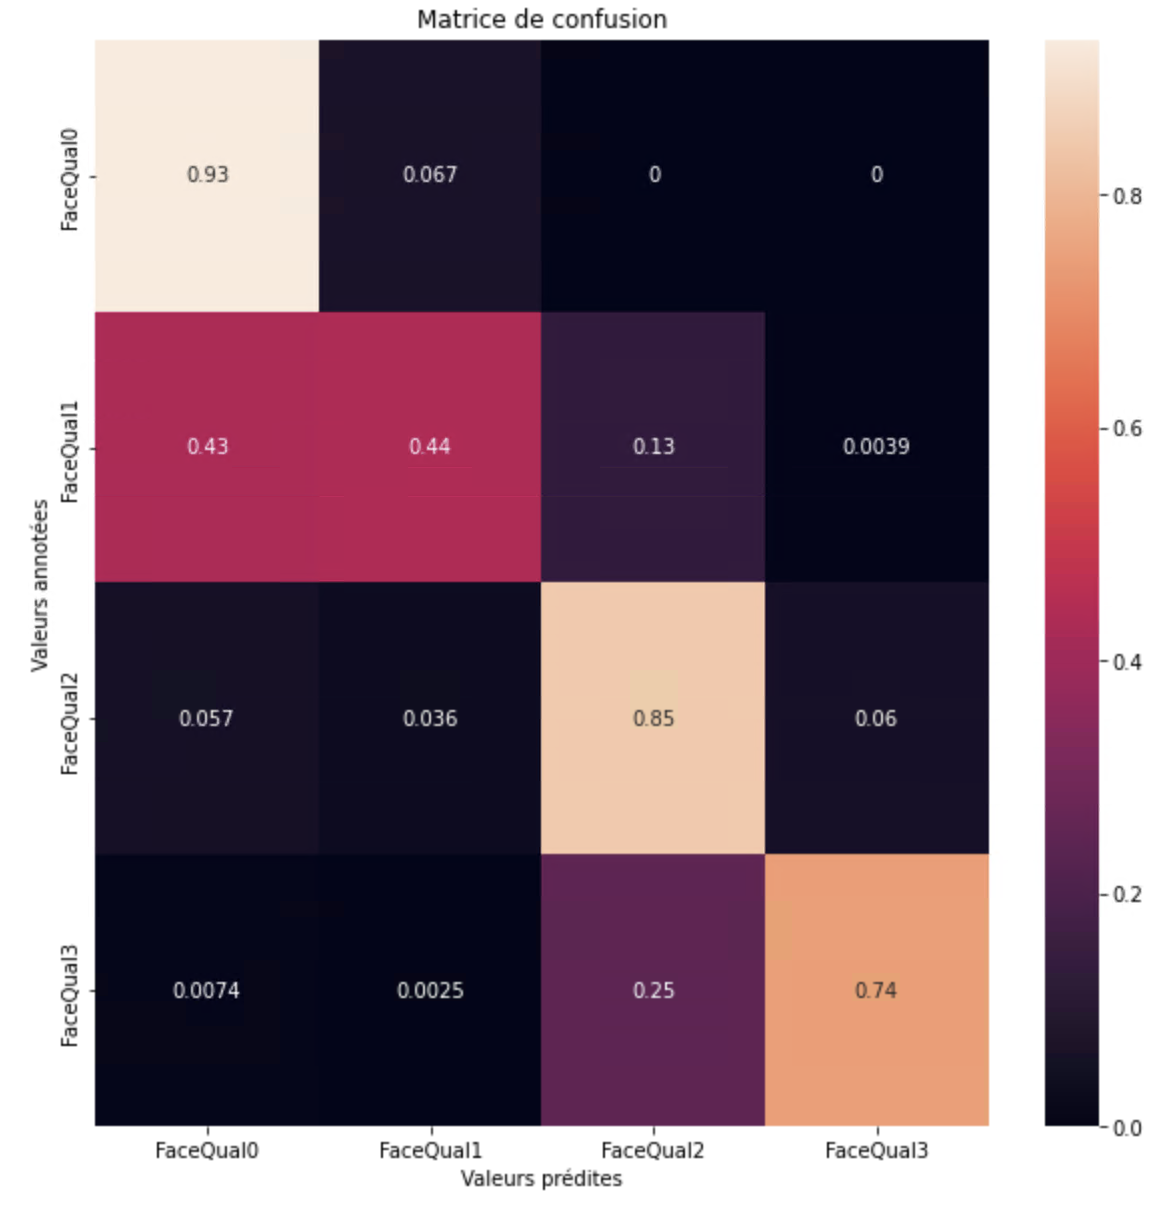
\includegraphics[width=170pt]{imgs/qualité/cr2/vgg16_010_confusion.png}
    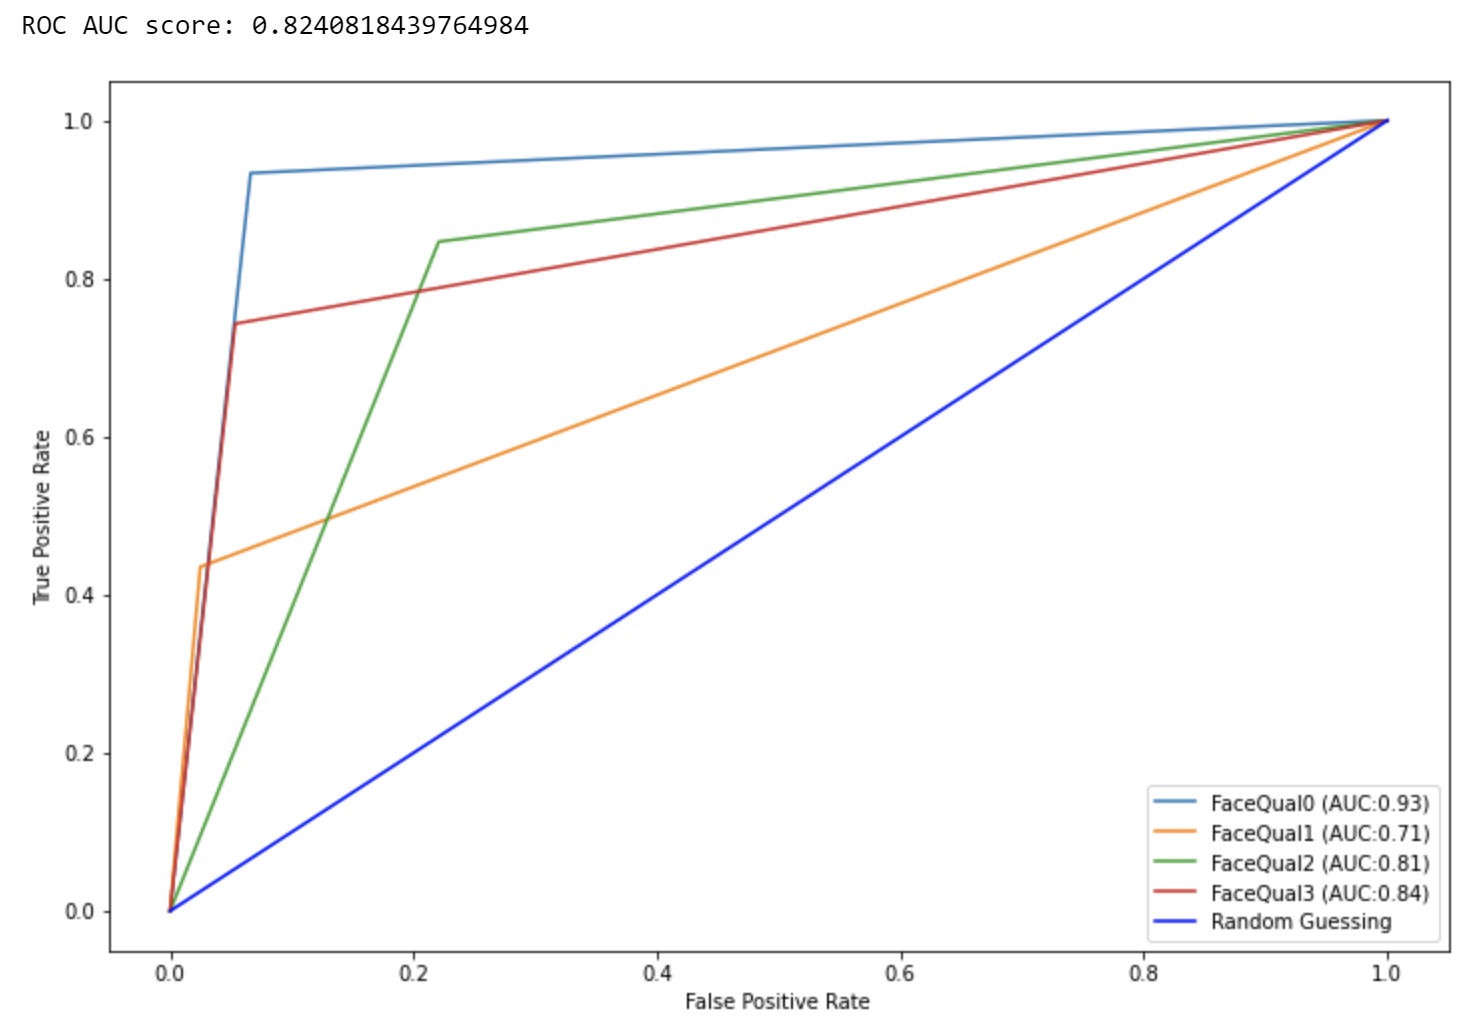
\includegraphics[width=170pt]{imgs/qualité/cr2/vgg16_010_roc.png}
\end{center}

Une piste est alors d'opérer un oversampling a priori sur la classe FaceQual0 pour avoir des poids de classes plus adéquats (moins grands). \\

Une fois testé, nous trouvons un rappel supérieur à la situation initiale sans cette fois-ci occasionner de dommages collatéraux. Le poids de la classe FaceQual0 après l'oversampling par copie/dégradation des images FaceQual3 est autour de 4, soit 4 fois moins qu'avant oversampling.

\begin{center}
    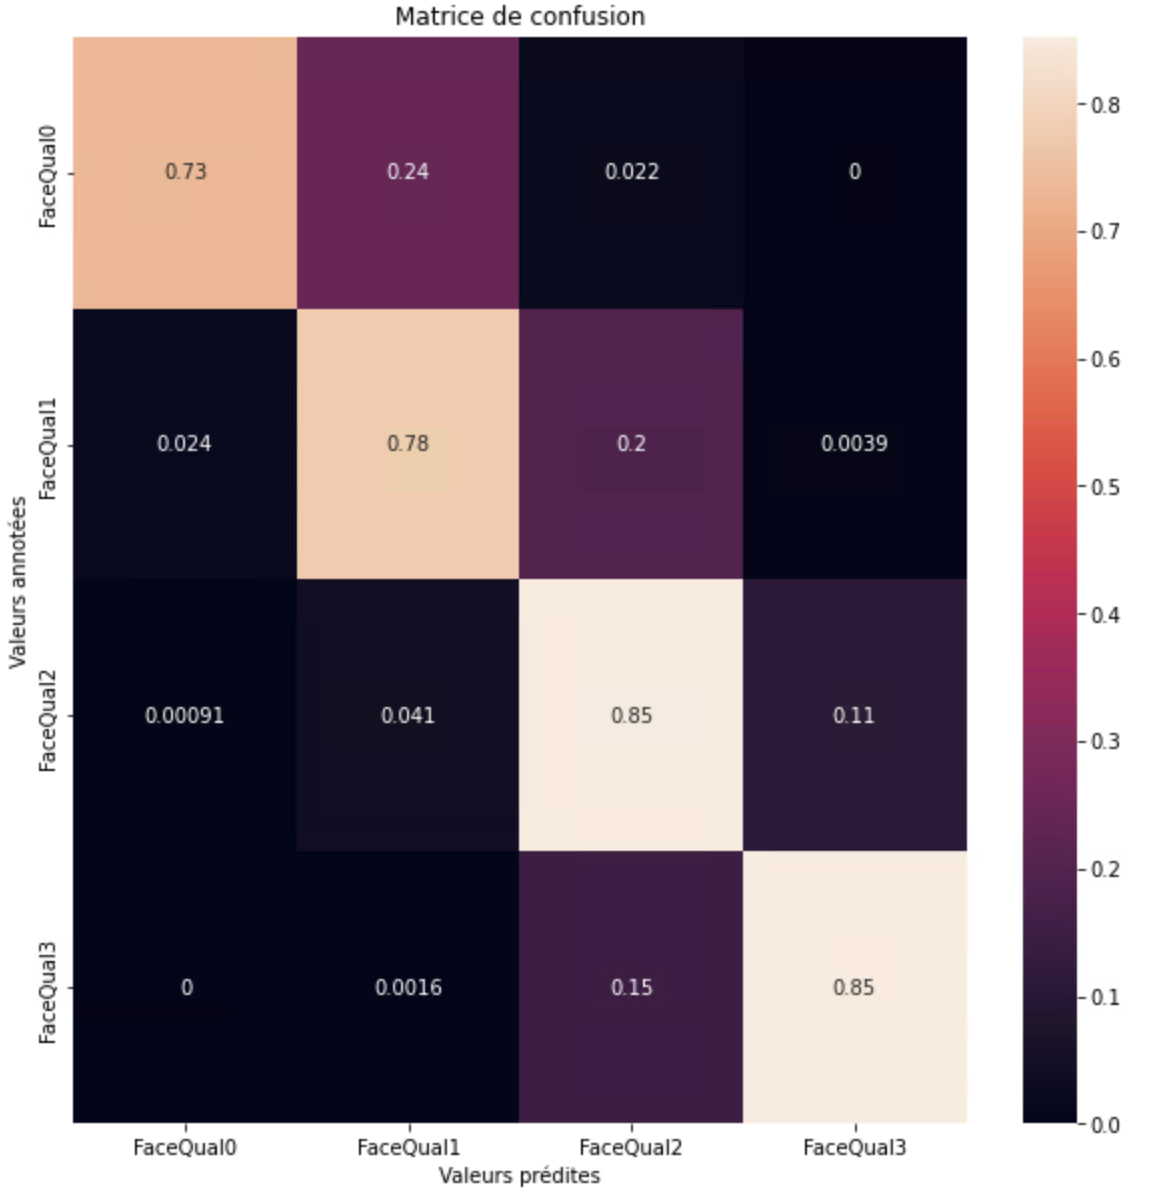
\includegraphics[width=170pt]{imgs/qualité/cr2/vgg16_011_confusion.png}
    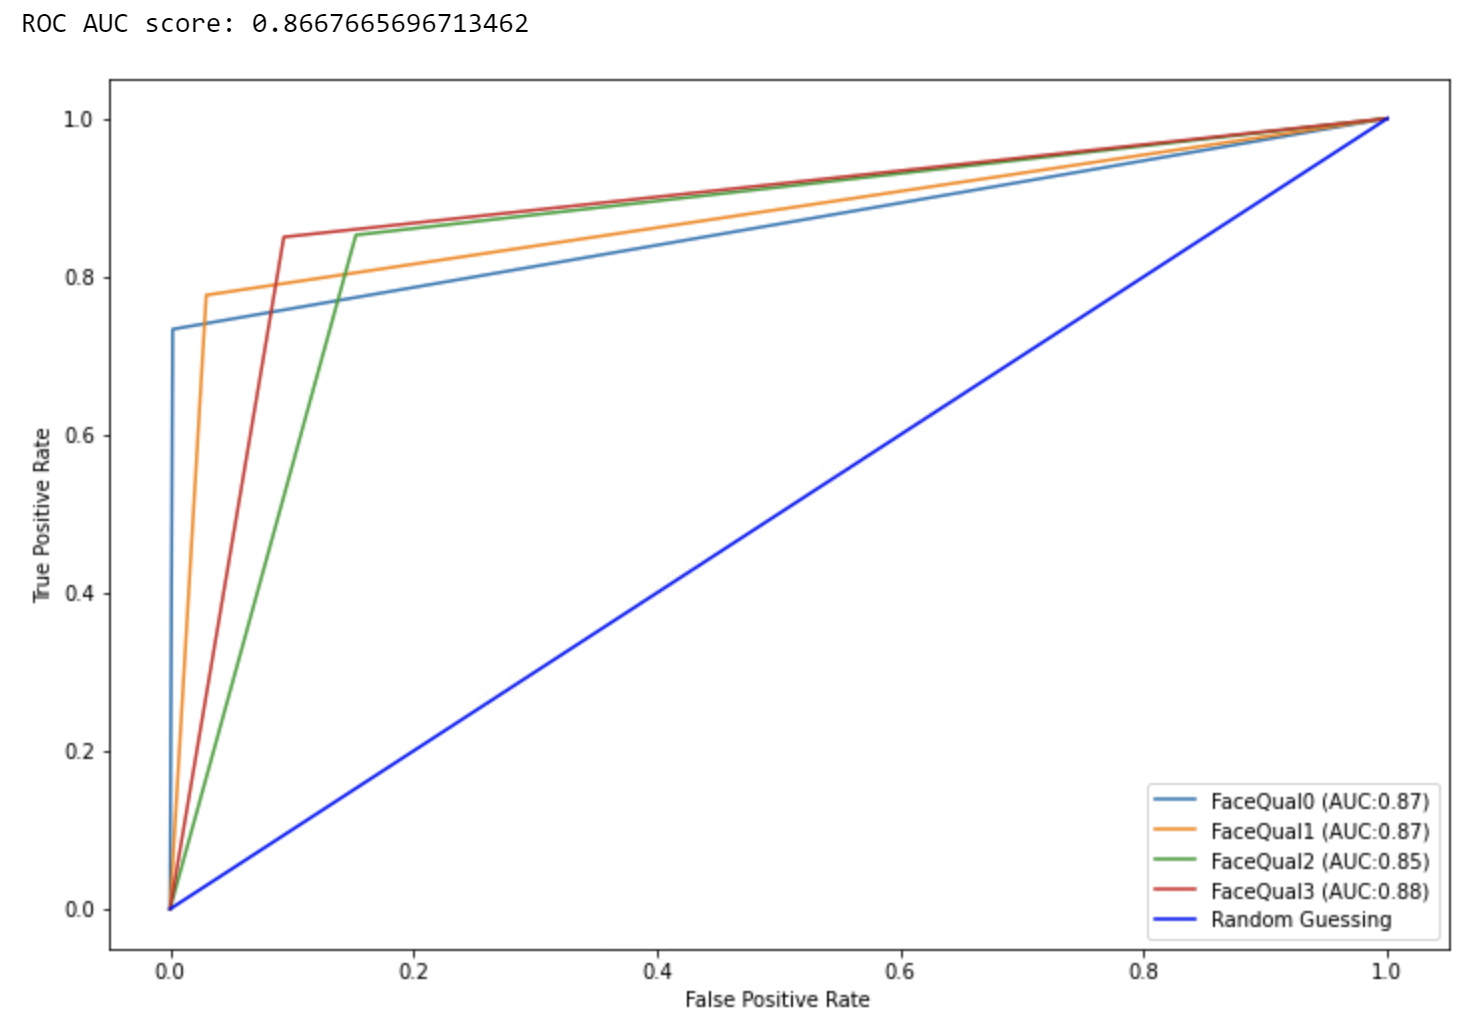
\includegraphics[width=170pt]{imgs/qualité/cr2/vgg16_011_roc.png}
\end{center}

\subsection{Base de données des métadonnées}
Avant le commencement du stage, les métadonnées étaient répartis sur plusieurs fichiers CSV. Cela induisait donc une certaine dureté pour y appliquer des modifications, ainsi qu'une rigidité pour utiliser les fichiers.\\

Alors nous nous sommes poser la question s'il pourrait être intéressant de créer une base de données pour organiser mieux le lien entre les métadonnées d'une image originale, d'une image portrait, d'un individu mandrill, etc...
Pour moi, le choix le plus cohérent était de partir sur une base de données SQLite, dite "file-based" (basé seulement sur le fichier). Ainsi, cela reste relativement simple à utiliser pour un centre de recherche non spécialisé en informatique puisqu'il n'y a pas de serveur, où tout le monde n'aurait pas envie de gérer ce dernier. Ce n'est pas non plus nécessaire car il n'y a pas réellement d'accès concurrent à cette base de données : elle sert avant tout pour les modèles d'entraînement ensuite.

\begin{center}
    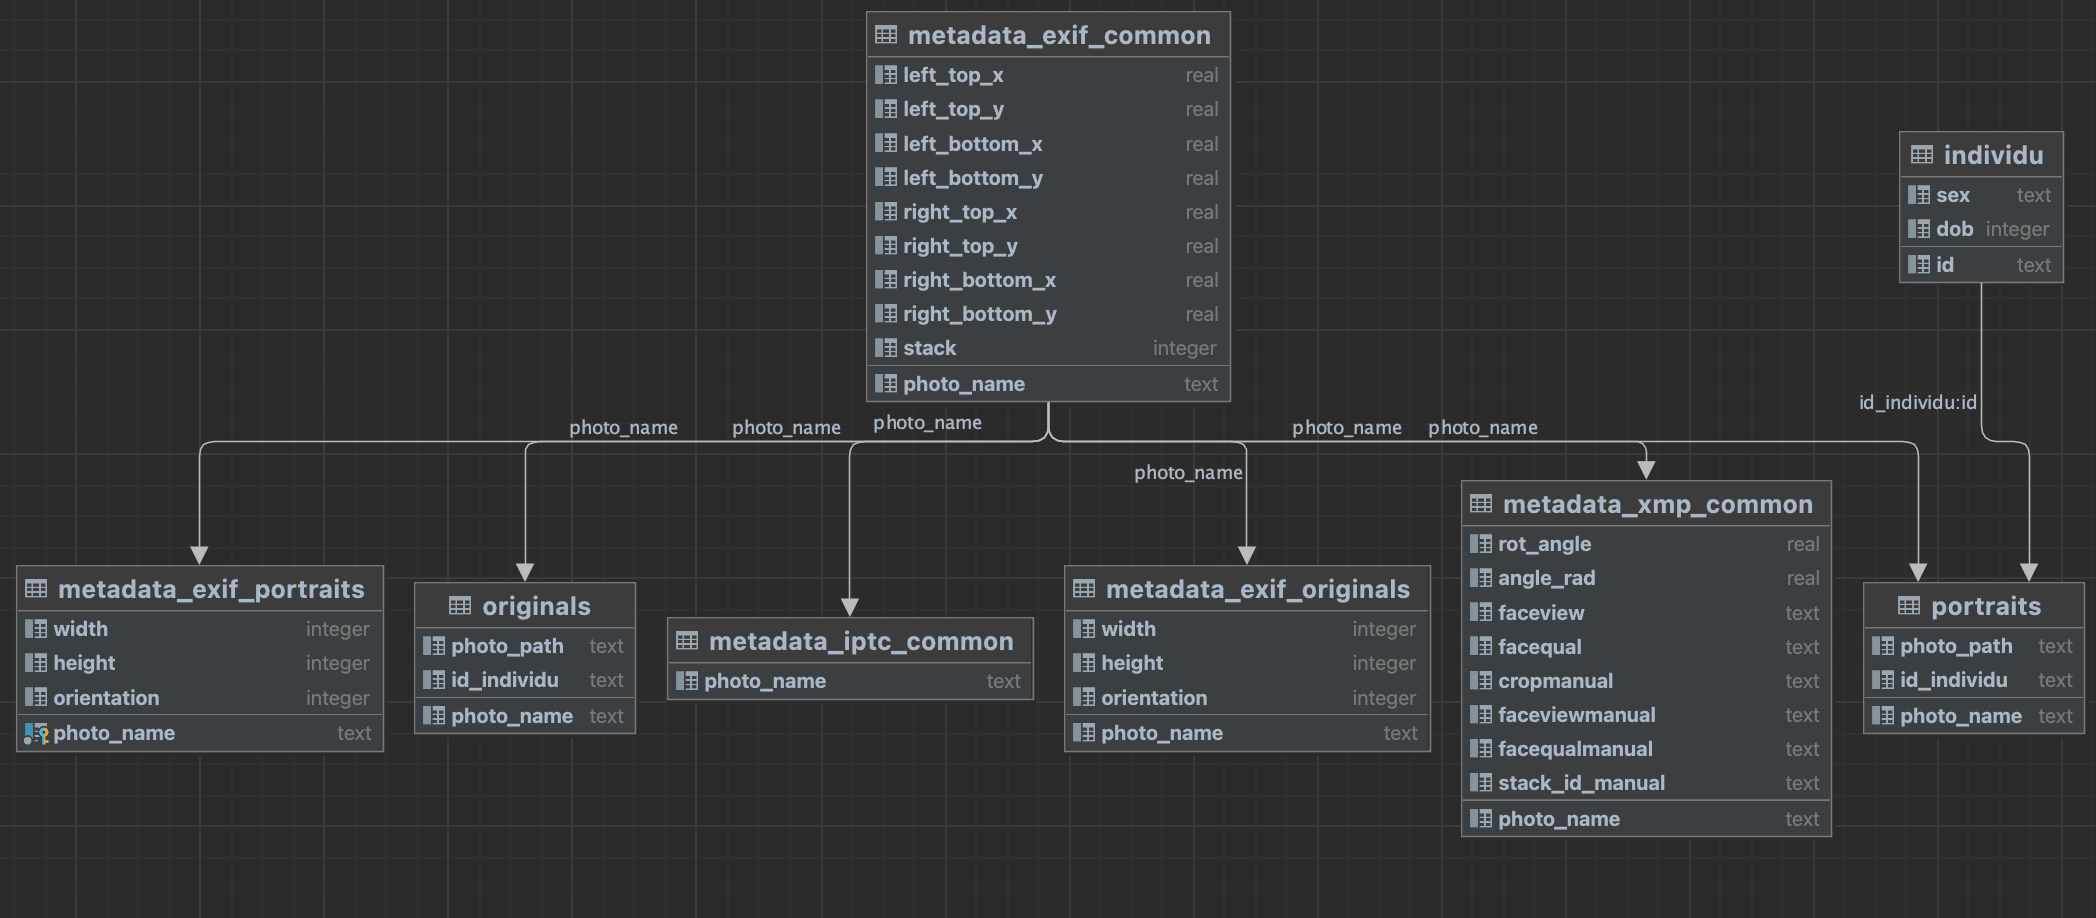
\includegraphics[width=345pt]{imgs/qualité/cr8/sqlite_schema.png}
\end{center}

\subsection{Docker}
Pour améliorer la portabilité de tous les scripts, j'ai mis en place Docker ainsi que Docker Compose. Docker est un logiciel qui permet de lancer un script avec son environnement "figé" de sorte qu'il fonctionne partout.\\

Voici donc des exemples de mes Dockerfile et docker-compose.yml : \\

Dans Dockerfile, nous précisions l'image de base (un OS ou, ici, un OS et une version de Python). Ensuite nous construisons l'image, en copiant les scripts locaux et installants les dépendances enregistrés dans un fichier requirements.txt (standard pour python pip). Enfin la commande ENTRYPOINT indique le point de départ de l'application, et CMD les paramètres par défaut, qui sont eux pour leur part surchargeables.
\begin{center}
    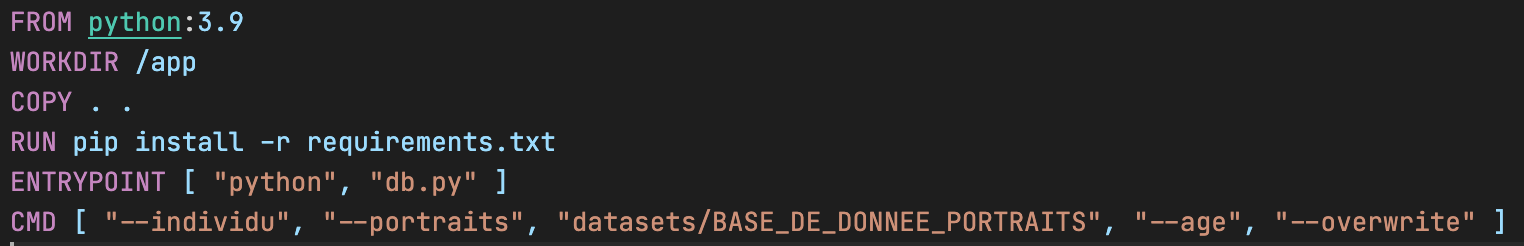
\includegraphics[width=345pt]{imgs/qualité/cr9/dockerfile.png}
\end{center}

Dans docker-compose.yml, nous pouvons composer des Dockerfile pour qu'ils soient dépendants les uns des autres ou simplement les lancer indépendamment des autres. Cela permet aussi de décrire les volumes / bind mounts directement dans un fichier de configuration (sans ces derniers les données seraient non persistantes).
\begin{center}
    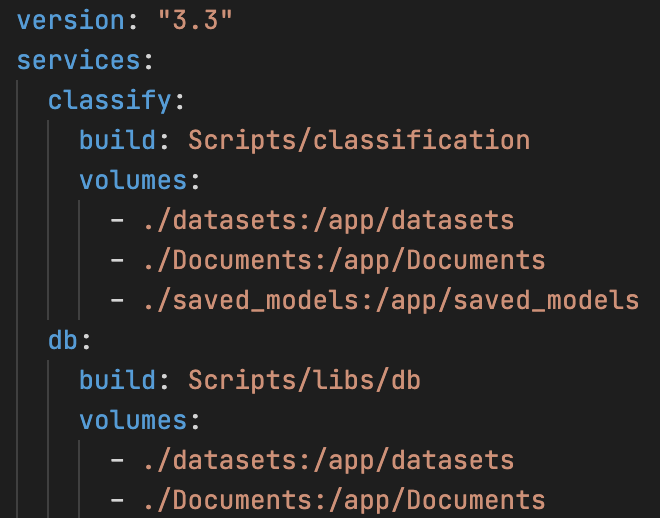
\includegraphics[width=345pt]{imgs/qualité/cr9/compose.png}
\end{center}

Voici un exemple de build des images et de run de l'image db. Comme le docker-compose indique l'utilisation de bind mounts, /app/Documents/Metadata/metadata.sqlite dans le container n'est autre que le fichier [projet]/Documents/Metadata/metadata.sqlite (persistant).
\begin{center}
    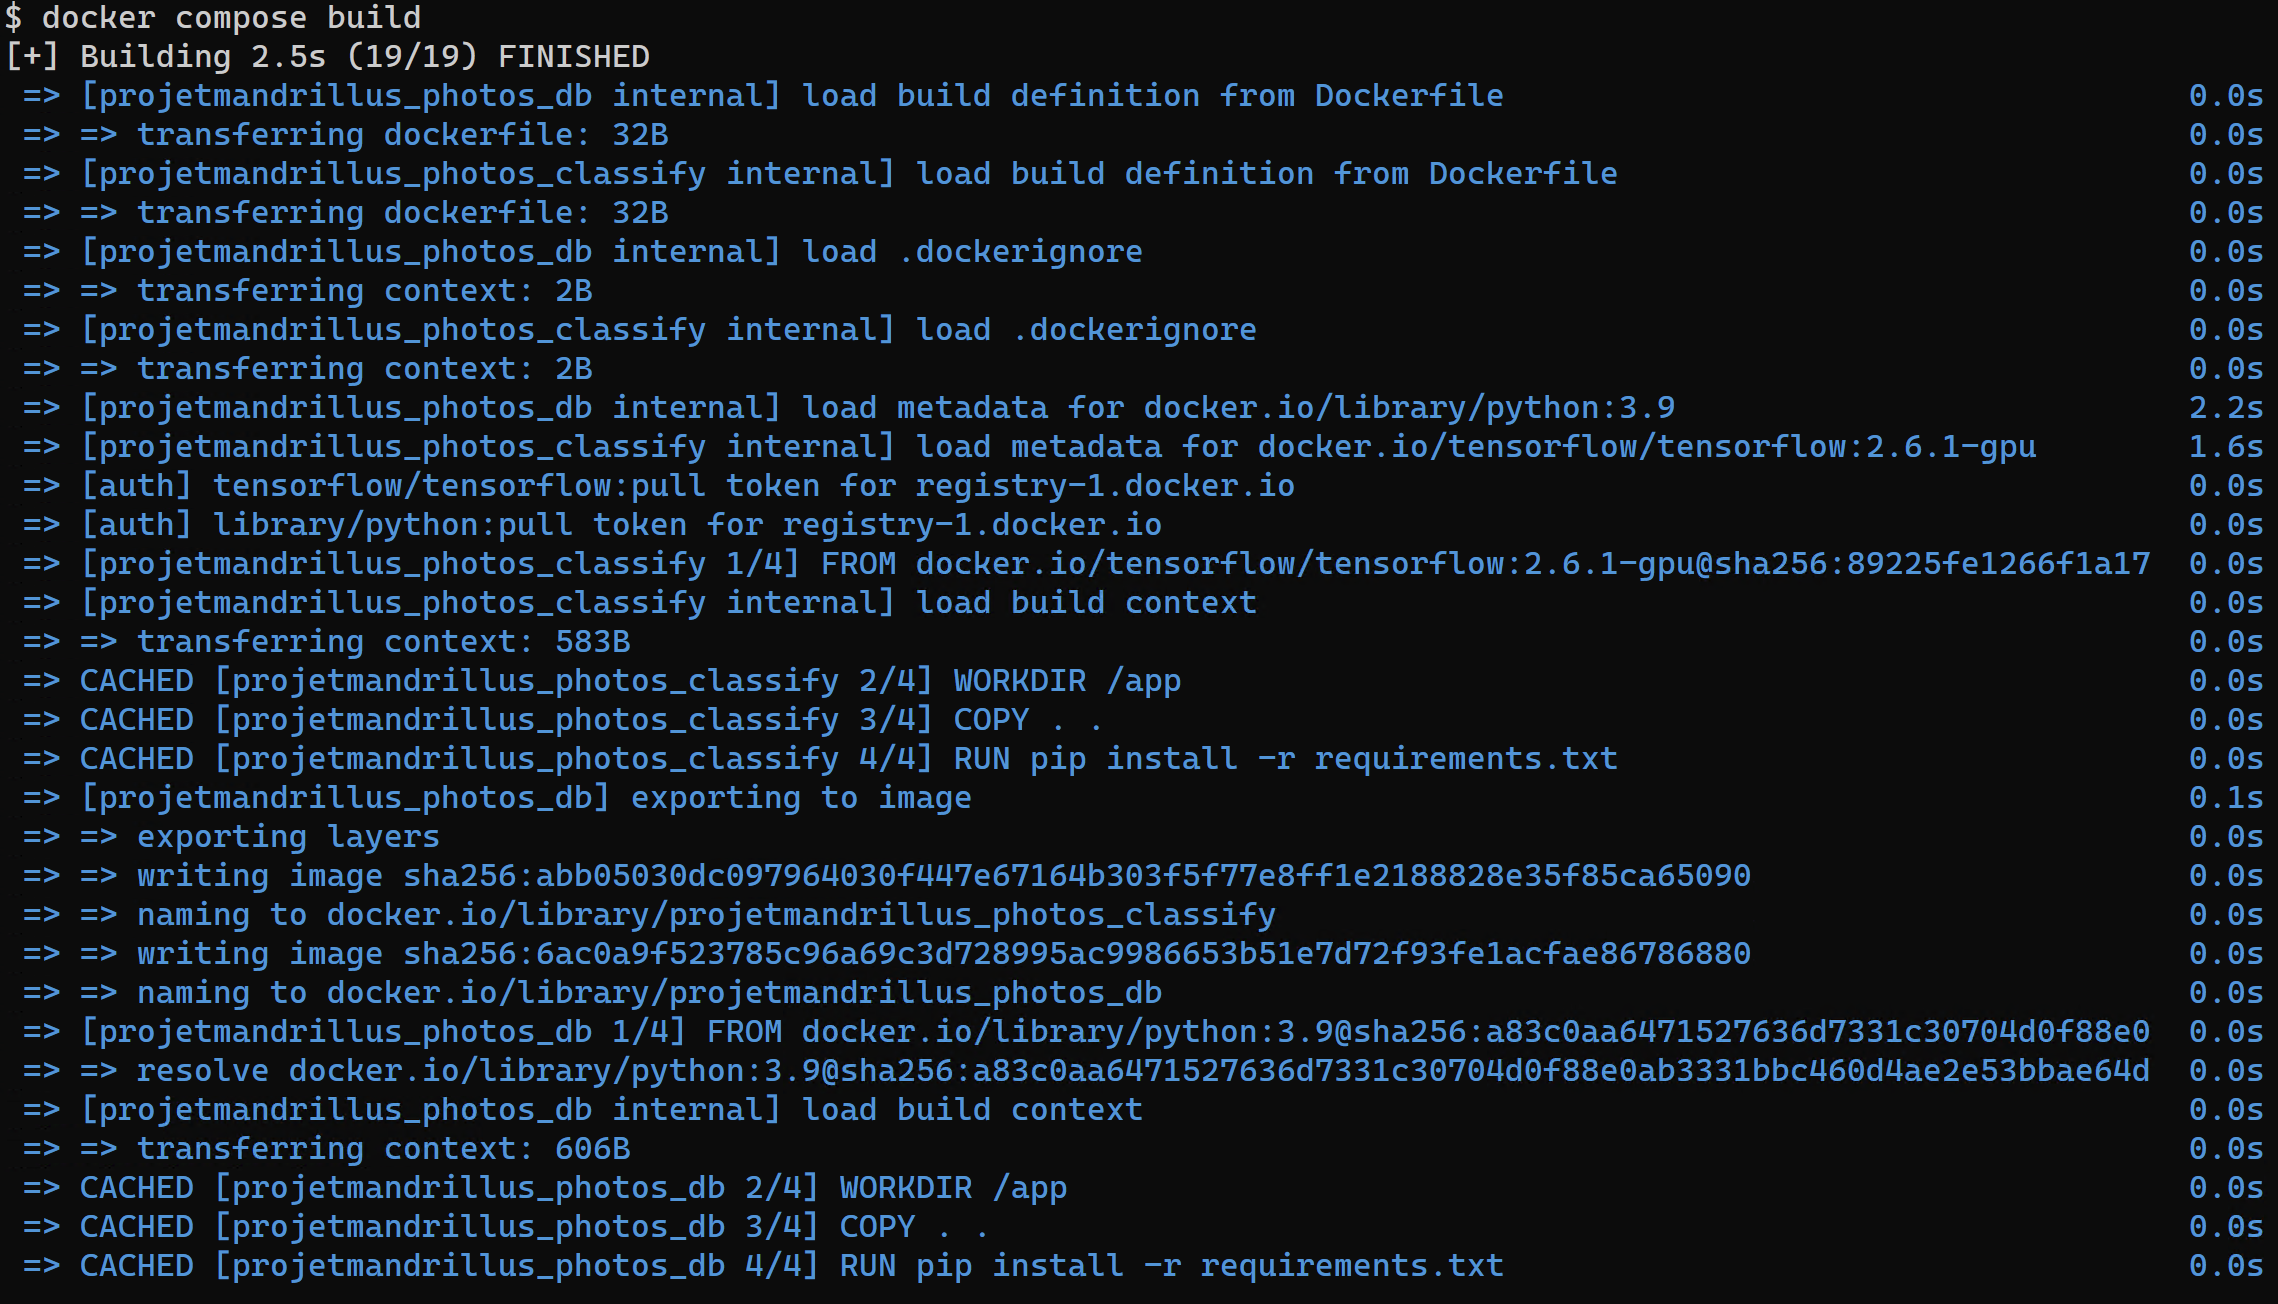
\includegraphics[width=345pt]{imgs/qualité/cr9/build.png}
    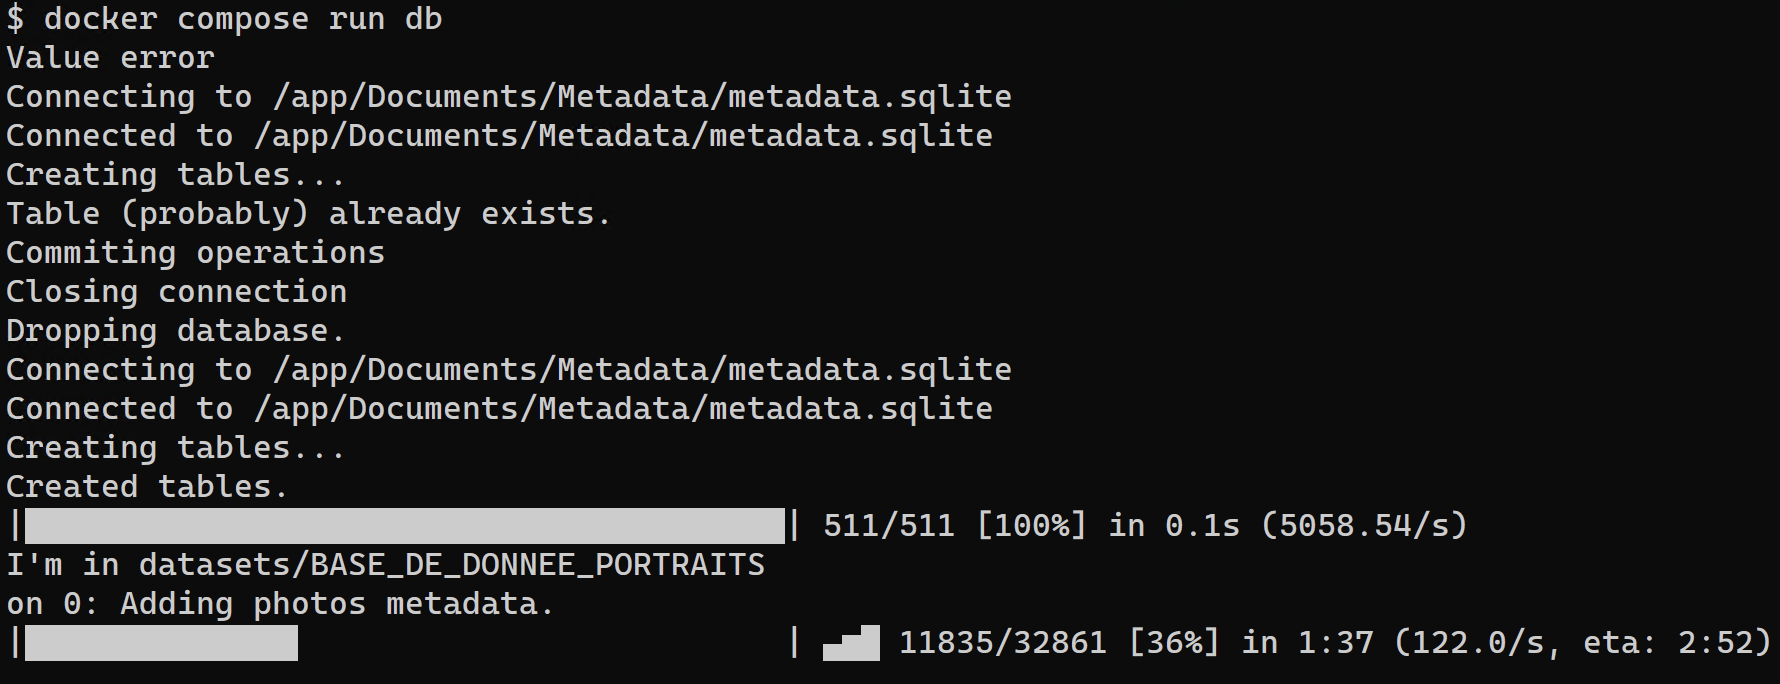
\includegraphics[width=345pt]{imgs/qualité/cr9/run.png}
\end{center}


\subsection{Tache 3}

\section{Conclusion}
Le stage m'a permis d'intégrer la méthode scientifique dans mon travail : rigueur au niveau des comparaisons et résultats. C'est donc une leçon qui a une très longue portée car cela me sera utile toute ma vie et peu importe le domaine. \\

Par ailleurs, j'en ai appris un peu plus sur le machine learning et les statistiques qui, là encore, présentent un intérêt dans plusieurs disciplines scientifiques. \\

J'ai également utilisé mes connaissances en gestion de projet, en particulier agile, en conservant un kanban personnel, et en faisant des réunions assez régulières (mais pas de mêlées quotidiennes), ainsi qu'en gérant le projet github.


\section{Glossaire}
\clearpage
\printglossary[title={Glossaire}]


\listoffigures

\section{Bibliographie} 
\printbibliography[
heading=subbibintoc,
title={ }
] 

\end{document}
